%The following is a template for including figures:

\begin{figure}[h]
\includegraphics[width=\textwidth]{<file_name>}
\caption{<caption>}
\label{fig:<figure_label>}
\end{figure}


% Figures from the paper will enter the document in the following order:




% 1. Decay diagrams
\begin{figure}[h]
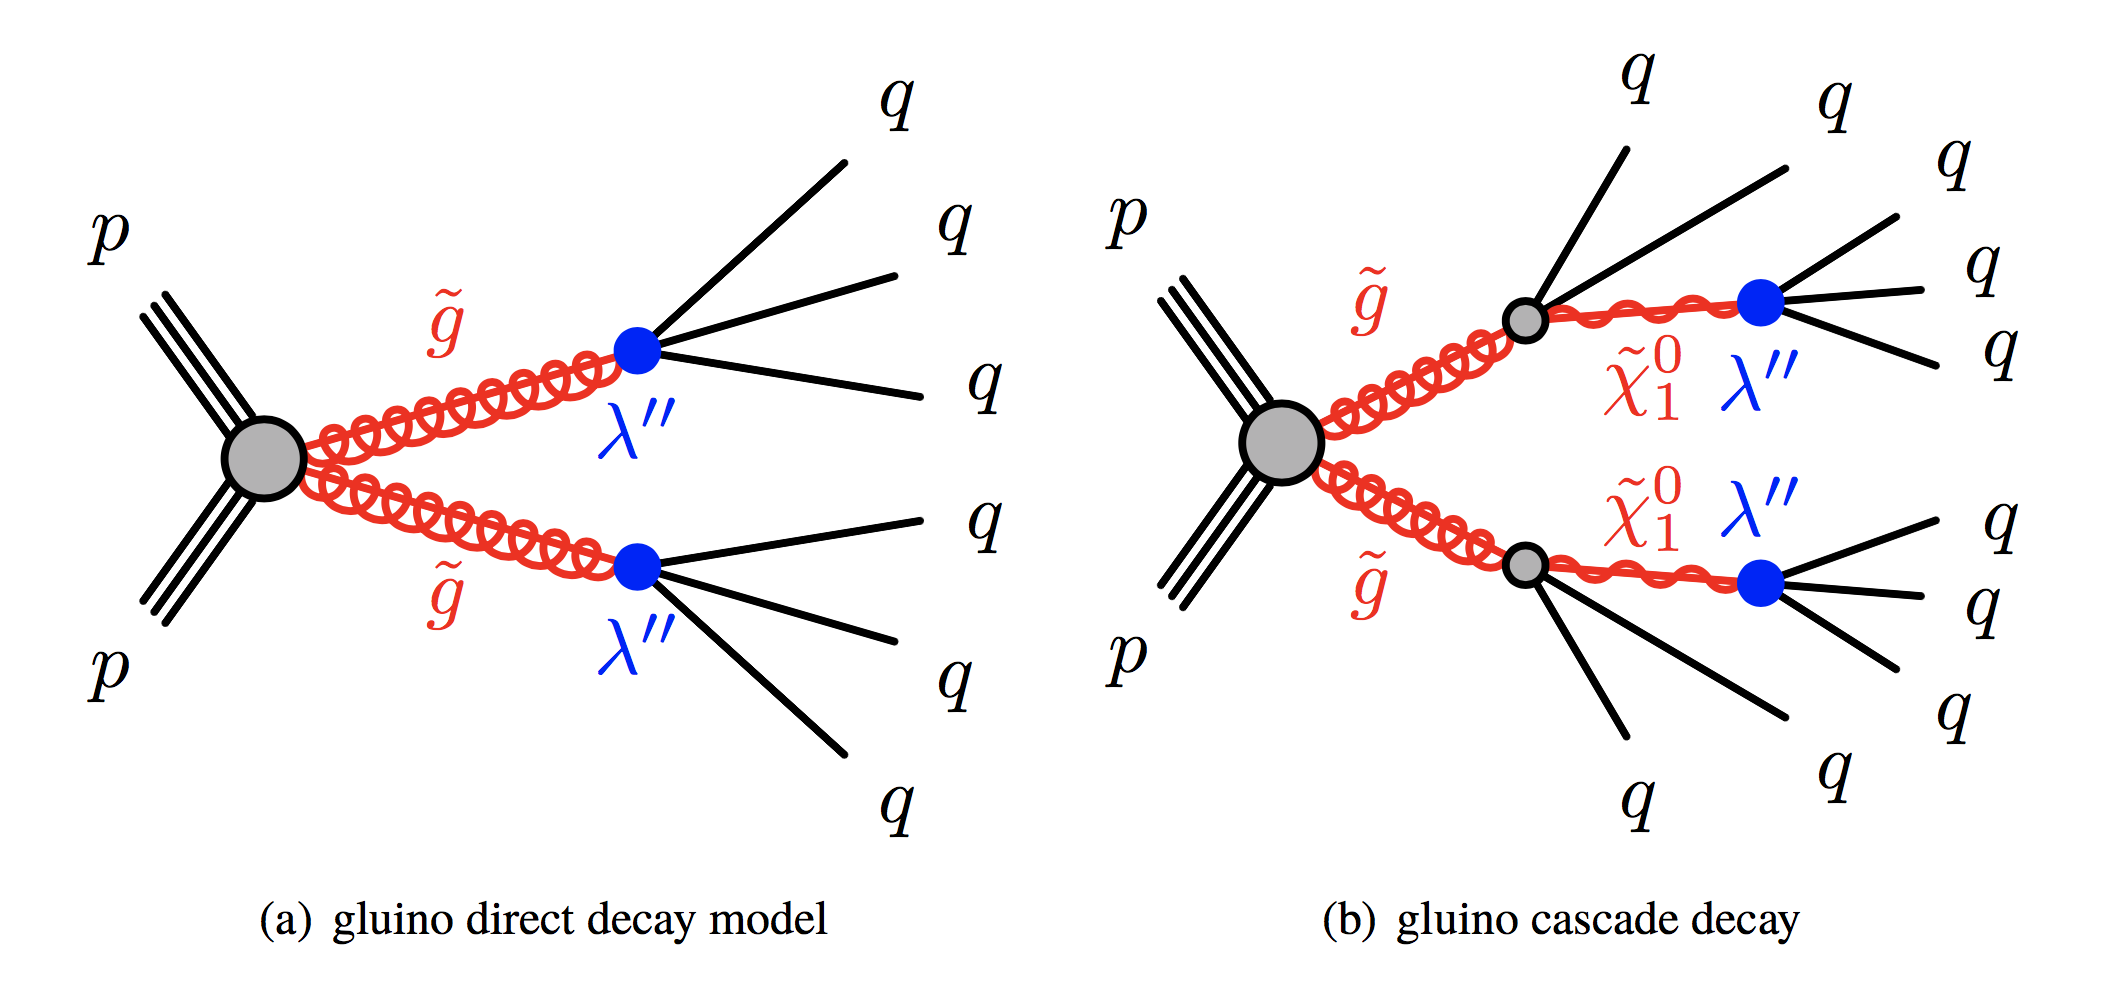
\includegraphics[width=\textwidth]{decay_diagrams_combined}
\caption{Diagrams illustrating the direct and cascade decay modes considered. The blue circles indicate the effective vertices, arising from an off-shell squark decaying to two quarks. At energies far below the squark mass, the contribution to the amplitude from each blue vertex is proportional to $\lambda''$.}
\label{fig:decay_diagrams}
\end{figure}

% 2. MJ / dEta distributions
\begin{figure}[h]
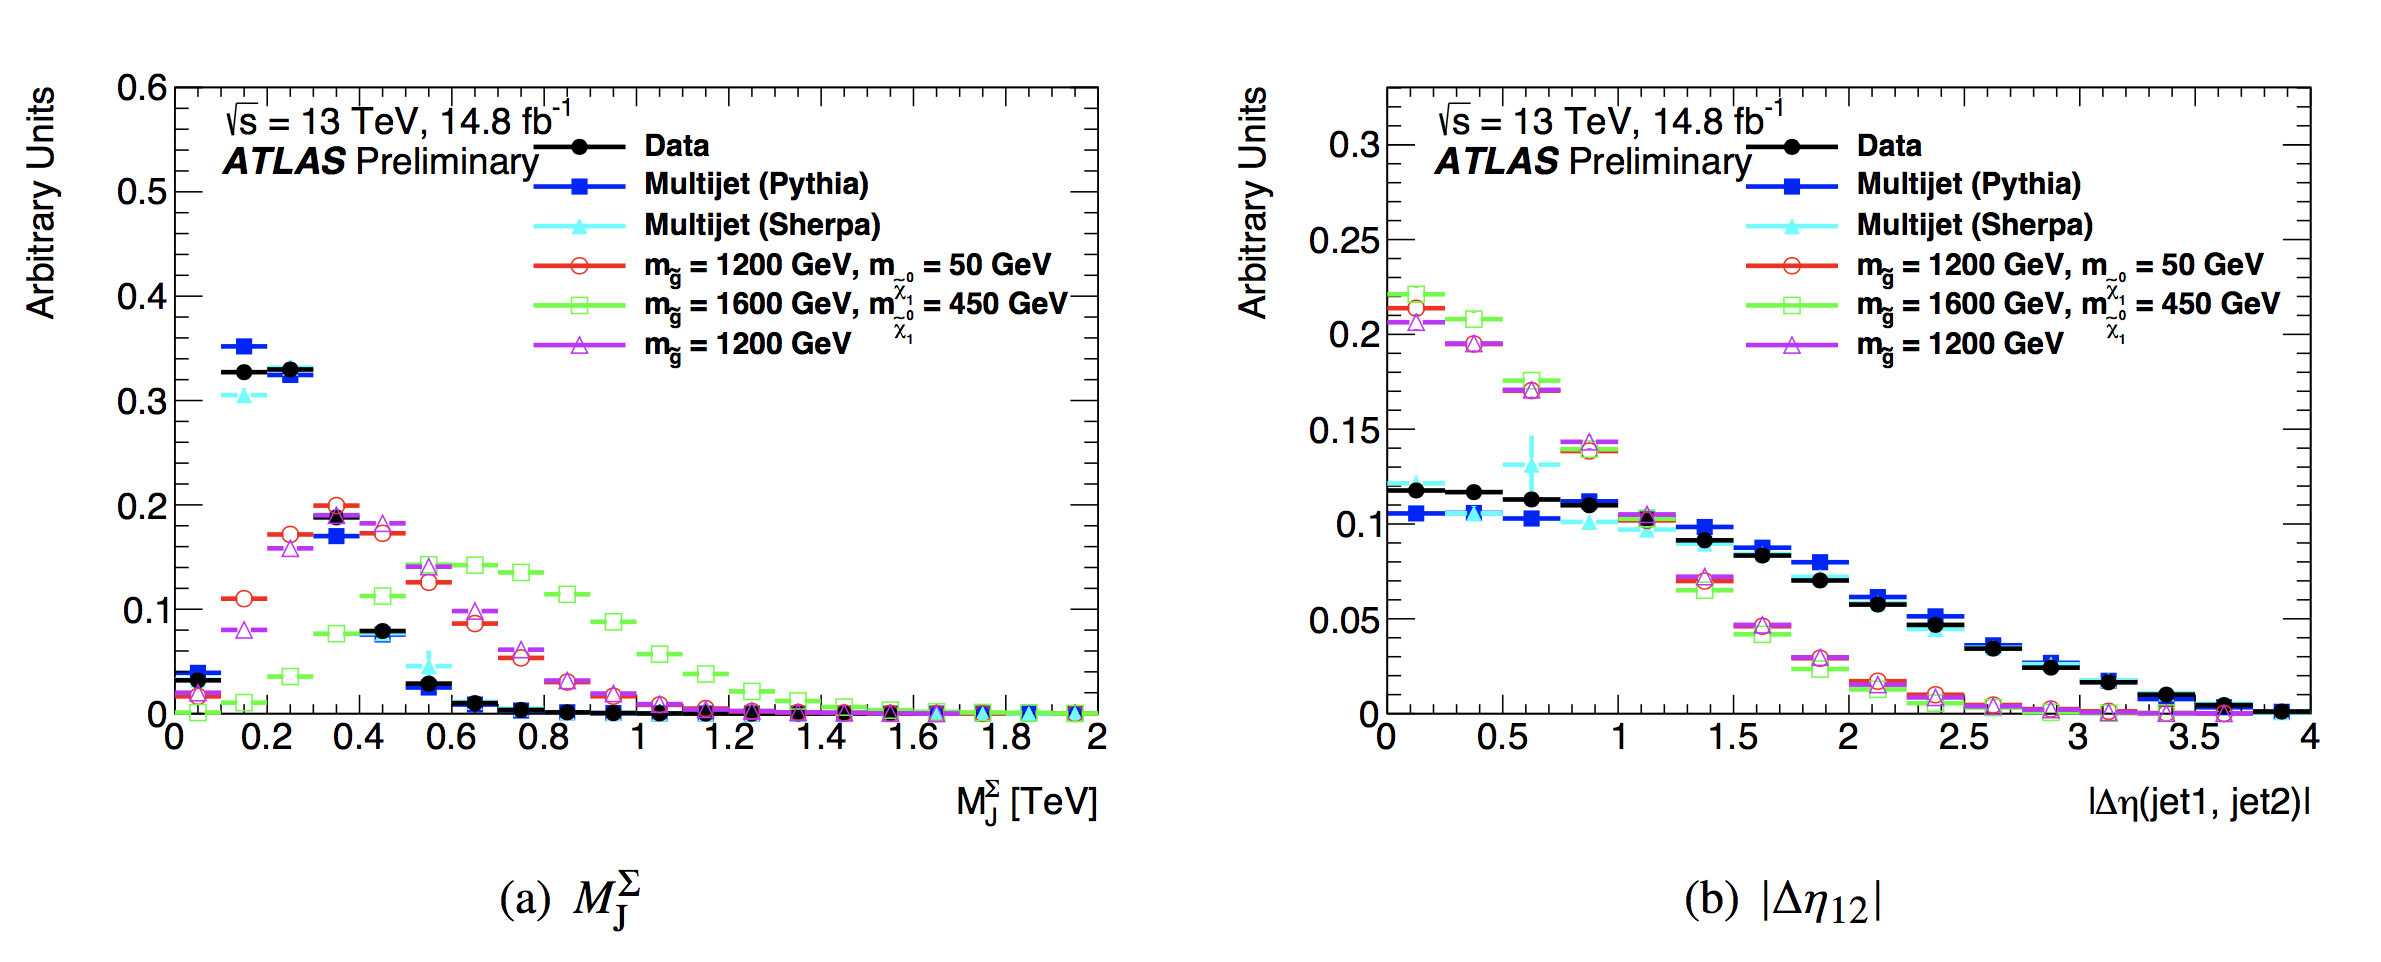
\includegraphics[width=\textwidth]{MJ_dEta_distributions_combined}
\caption{Distributions of the two main discriminating observables, (a) the scalar sum of the four leading large-R jets, $M_{J}^{\Sigma}$ and (b) the difference in pseudorapidity between the two leading jets, $|\Delta\eta_{12}|$. Selected events have $\geq 4$ large-R jets. Distributions are shown for both data and simulated signal and background samples. The red and green signal distributions are for the cascade decay mode, and the violet distribution is the direct decay mode, for the superpartner masses indicated.}
\label{fig:MJ_dEta_distributions}
\end{figure}

% 3. Observed MJ distributions, VRs
\begin{figure}[h]
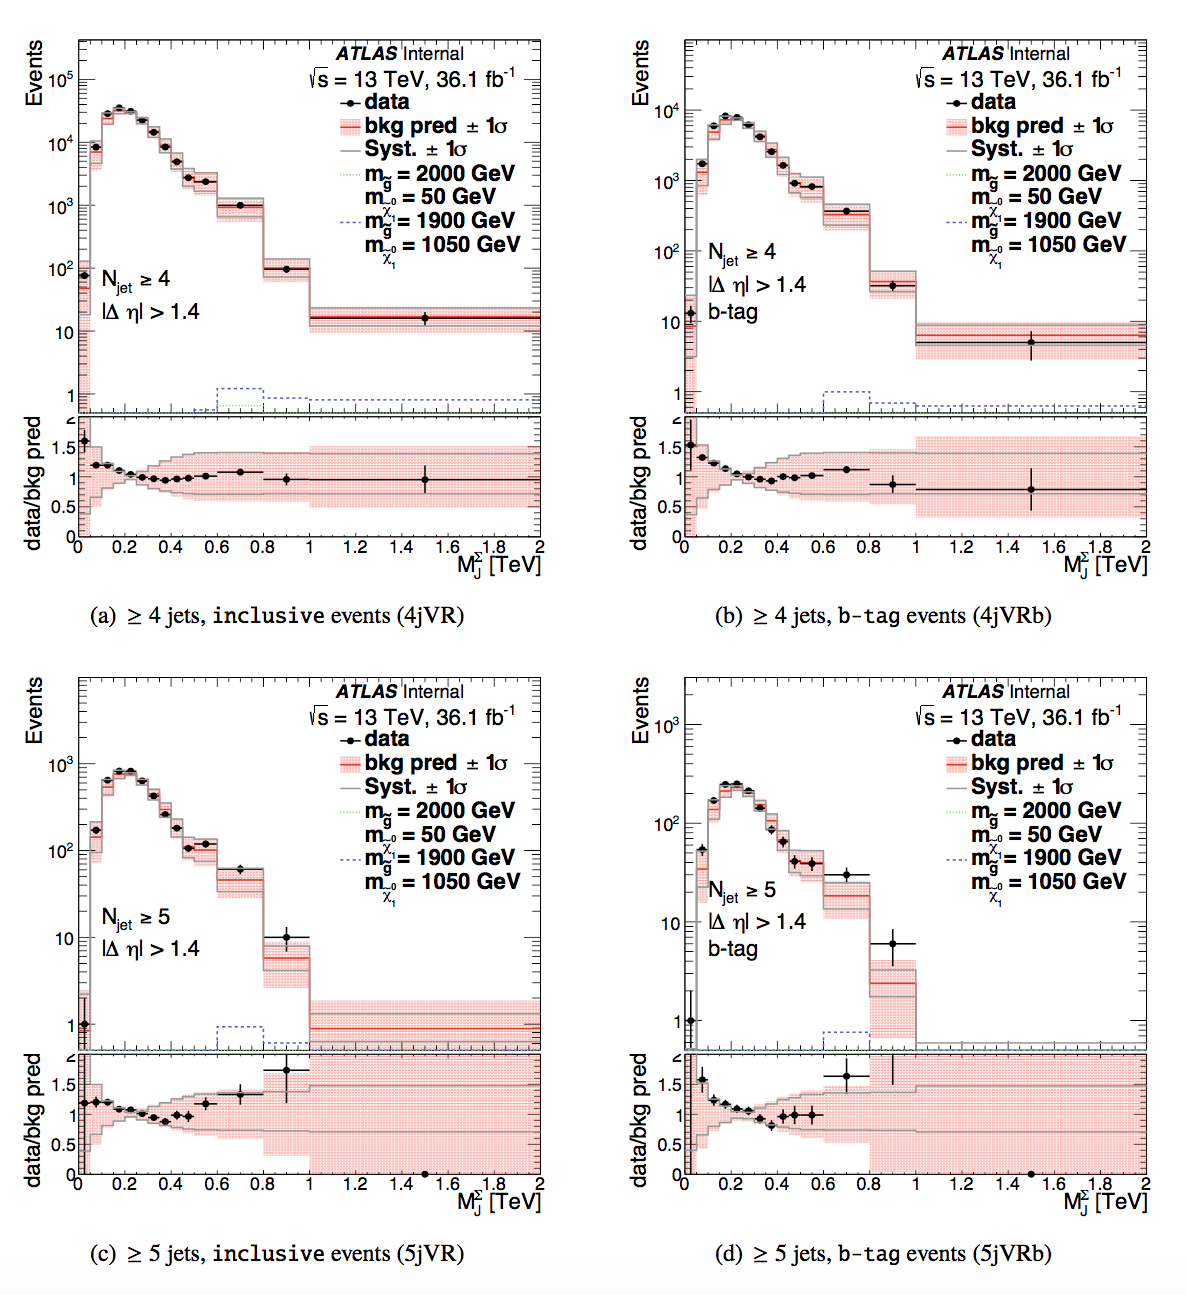
\includegraphics[width=\textwidth]{predicted_and_observed_MJ_VRs}
\caption{}
\label{fig:pred_obs_MJ_VRs}
\end{figure}

% 4. Observed MJ distribtuions, SRs
% 5. Limit plots

